
\begin{frame}[c]
  \frametitle{Case III : Solubility Coefficient}
The dissolution behavior of a solute in an aqueous solutions is called its 
\textbf{solubility}. This behavior is limited by the solute's solubility limit, described  
by an equilibrium constant that depends upon temperature, water chemistry, and 
the properties of the element. The solubility constant for ordinary solutes, 
$K_s$ gives units of concentration, $[kg/m^3]$, and can be determined 
algebraically by the law of mass action which gives the partitioning at 
equilibrium between reactants and products.  For a reaction
\begin{align}
  cC + dD &= yY + zZ,
  \intertext{where}
  c,d,y,z  &= \mbox{ amount of respective constituent }[mol]\nonumber\\
  C,D  &= \mbox{ reactants }[-]\nonumber\\
  Y,Z  &= \mbox{ products }[-]\nonumber,
  \intertext{the law of mass action gives}
  K &= \frac{(Y)^y(Z)^z}{(C)^c(D)^d}
  \intertext{where}
  (X)  &= \mbox{ the equilibrium molal concentration of X }[mol/m^3]\nonumber\\
  K  &= \mbox{ the equilibrium constant }[-].\nonumber
  \label{massaction}
\end{align}
\end{frame}

\begin{frame}[c]
  \frametitle{Case III : Solubility Coefficient}
The reference solubilities for each element were multiplied by the multiplier 
for each simulation group. This technique preserved relative solubility among 
  elements. 

\begin{table}[ht!]
\centering
\footnotesize{
\begin{tabular}{|l|l|l|r|r|}
\multicolumn{5}{c}{\textbf{Simulation Cases}}\\
\hline
\textbf{Case} & \textbf{Parameter} & \textbf{Units} & \textbf{Min. Value} & \textbf{Max. Value}\\
\hline
III   & $S_i$        & $[mol\cdot m^{-3}]$       & $(1\times10^{-9})\langle S_i\rangle $    &  $(5\times10^{10})\langle S_i\rangle $ \\
\hline
\end{tabular}
\caption{Case III varied a solubility factor across many magnitudes. This single parameter simulation case had 40 simulation 
groups of 100 realizations each.}
\label{tab:Cases}
}
\end{table}


\end{frame}


\begin{frame}[c]
  \frametitle{Case III : Solubility Coefficient}
The results for varying the solubility coefficient were very straightforward.  
For solubility limits below a certain threshold, the dose releases were directly 
proportional to the solubility limit, indicating that the radionuclide 
concentration saturated the groundwater up to the solubility limit near the 
waste form.  For solubility limits above the threshold, however, further 
increase to the limit had no effect on the peak dose. This demonstrates the 
situation in which the solubility limit is so high that even complete 
dissolution of the waste inventory into the pore water is insufficient to reach 
the solubility limit.
\end{frame}

\begin{frame}[c]
  \frametitle{Case III : Solubility Coefficient}


\begin{figure}[ht]
\centering
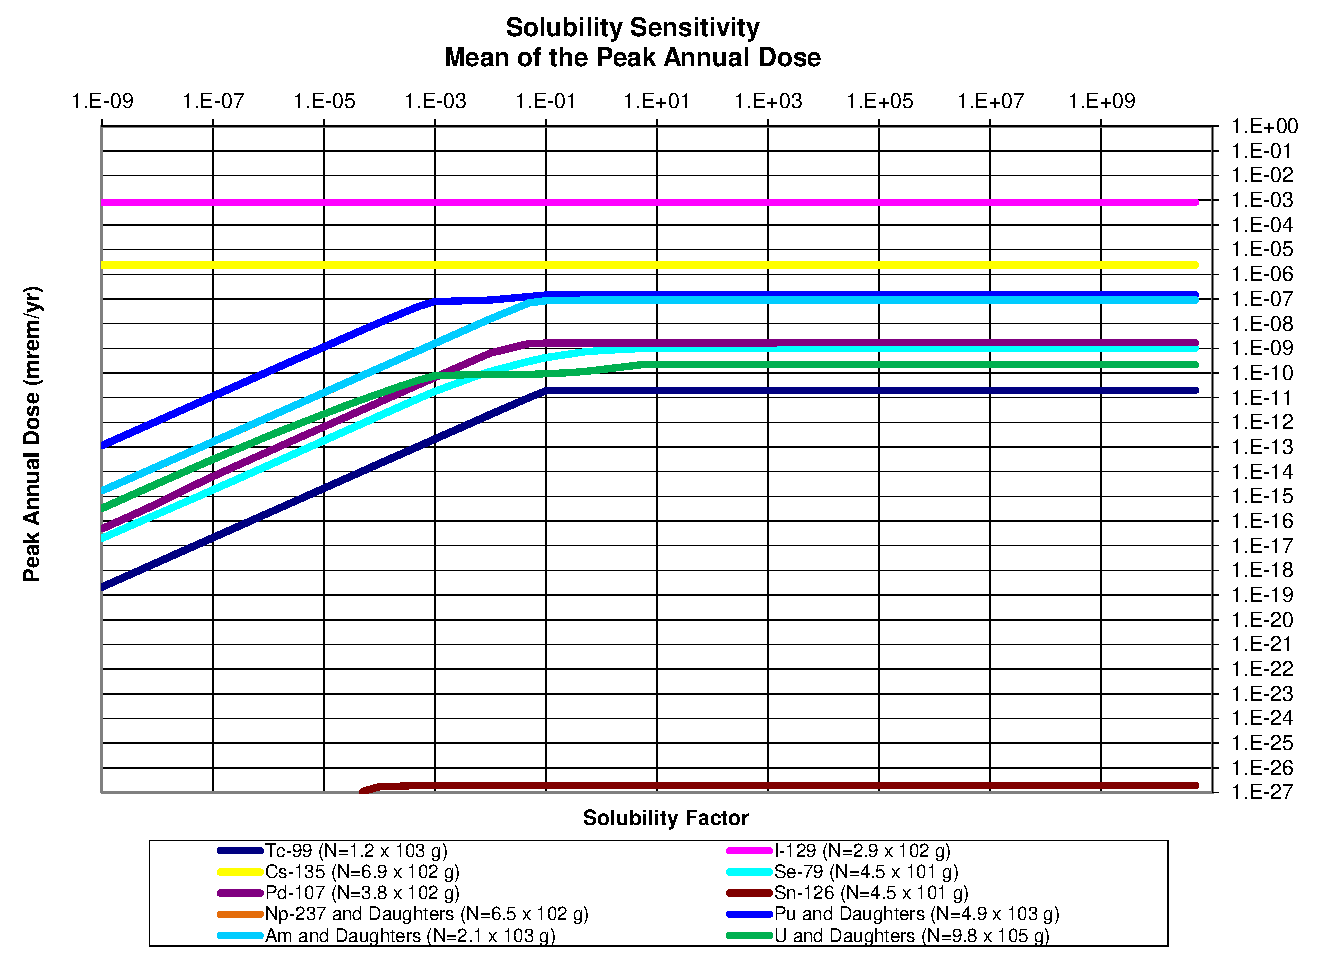
\includegraphics[width=\linewidth]{Solubility/Solubility_Summary_SolFactor.eps}
\caption{
The peak annual dose due to an inventory, $N$, of each isotope.
For solubility constants lower than the inventory threshold, the relationship between peak 
annual dose and solubility limit is strong.}
\label{fig:SolSumFactor}
\end{figure}
\end{frame}

\begin{frame}[c]
  \frametitle{Case III : Solubility Coefficient}

\begin{figure}[ht]
\centering
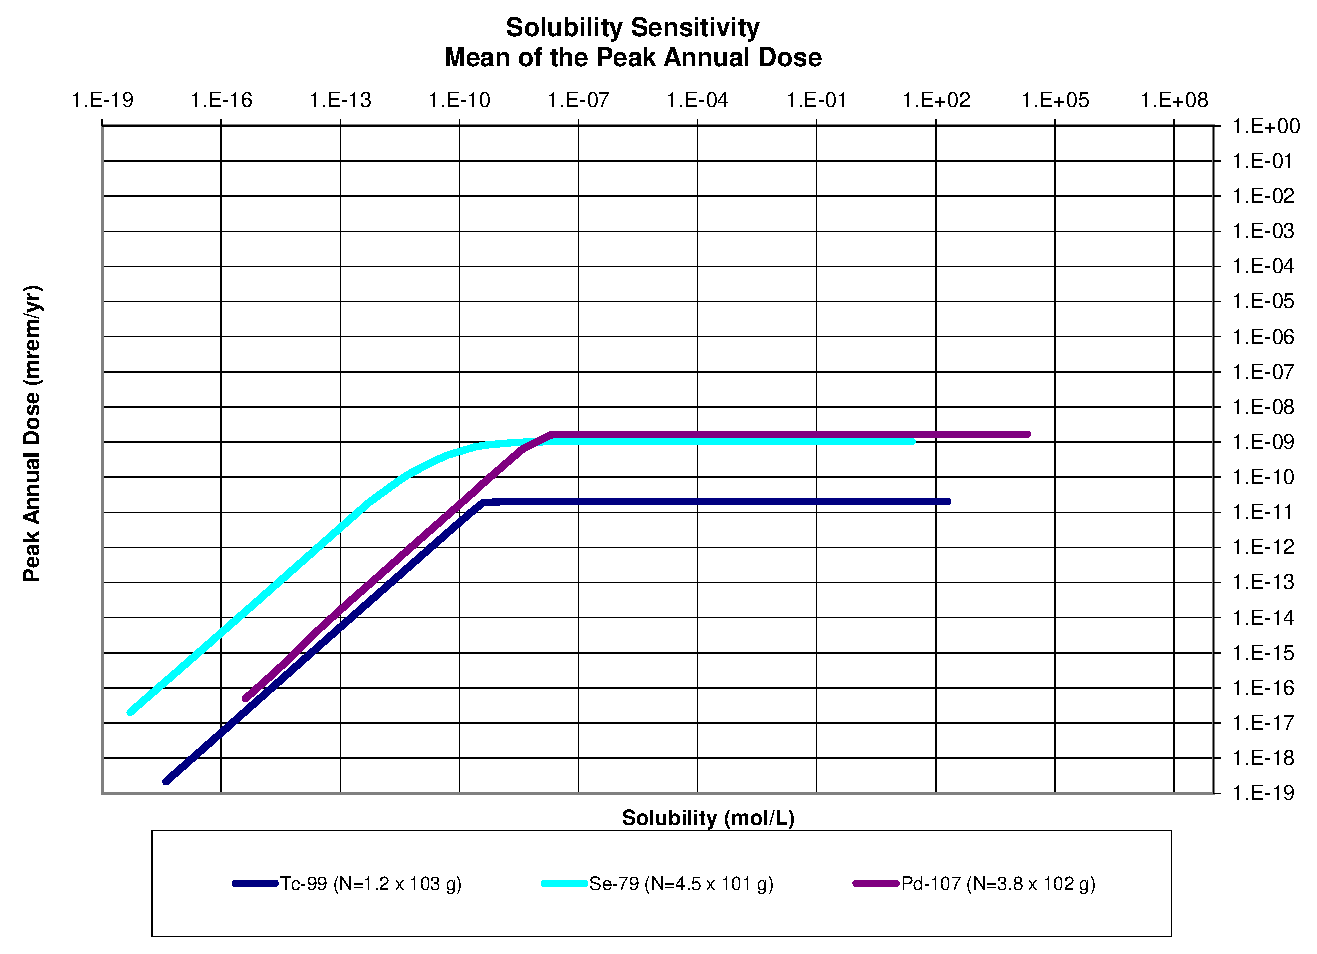
\includegraphics[width=\linewidth]{Solubility/Solubility_Summary_Sol.eps}
\caption{
The peak annual dose due to an inventory, $N$, of each isotope.
For solubility constants lower than the inventory threshold, the relationship between peak 
annual dose and solubility limit is strong.}
\label{fig:SolSum}
\end{figure}
\end{frame}

